%% Adaptado a partir de :
%%    abtex2-modelo-trabalho-academico.tex, v-1.9.2 laurocesar
%% para ser um modelo para os trabalhos no IFSP-SPO

\documentclass[
    % -- opções da classe memoir --
    12pt,               % tamanho da fonte
    openright,          % capítulos começam em pág ímpar (insere página vazia caso preciso)
    %twoside,            % para impressão em verso e anverso. Oposto a oneside
    oneside,
    a4paper,            % tamanho do papel. 
    % -- opções da classe abntex2 --
    %chapter=TITLE,     % títulos de capítulos convertidos em letras maiúsculas
    %section=TITLE,     % títulos de seções convertidos em letras maiúsculas
    %subsection=TITLE,  % títulos de subseções convertidos em letras maiúsculas
    %subsubsection=TITLE,% títulos de subsubseções convertidos em letras maiúsculas
    % Opções que não devem ser utilizadas na versão final do documento
    %draft,              % para compilar mais rápido, remover na versão final
    MODELO,             % indica que é um documento modelo então precisa dos geradores de texto
    TODO,               % indica que deve apresentar lista de pendencias 
    % -- opções do pacote babel --
    english,            % idioma adicional para hifenização
    brazil              % o último idioma é o principal do documento
    ]{ifsp-spo-inf-cemi} % ajustar de acordo com o modelo desejado para o curso
        
% ---

% --- 
% CONFIGURAÇÕES DE PACOTES
% --- 
%\usepackage{etoolbox}
%\patchcmd{\thebibliography}{\chapter*}{\section*}{}{}


% ---
% Informações de dados para CAPA e FOLHA DE ROSTO
% ---
\titulo{PROPOSTA INICIAL - IFRIENDS: COMUNIDADE DE APOIO AOS ALUNOS}

\renewcommand{\imprimirautor}{
\begin{tabular}{lr}
ANAÍ VILLCA ROJAS & SP3029085 \\
JAMILLI VITÓRIA GIOIELLI & SP3027473 \\
JOSÉ ROBERTO CLAUDINO FERREIRA & SP3024369 \\
JULIA ROMUALDO PEREIRA & SP3023061 \\
KAIKY MATSUMOTO SILVA & SP185075X \\
\end{tabular}
}


\tipotrabalho{Projeto da Disciplina de PDS}

\disciplina{PDS - Prática para Desenvolvimento de Sistemas}

\preambulo{Proposta de projeto de sistema para disciplina de PDS}

\data{2022}

\renewcommand{\orientadorname }{Professor:}
\coorientador{Carlos Henrique Veríssimo Pereira}
\renewcommand{\coorientadorname}{Professor:}
\orientador{Johnata Souza Santicioli}


% informações do PDF
\makeatletter
\hypersetup{
        %pagebackref=true,
        pdftitle={\@title}, 
        pdfauthor={\@author},
        pdfsubject={\imprimirpreambulo},
        pdfcreator={LaTeX with abnTeX2},
        pdfkeywords={abnt}{latex}{abntex}{abntex2}{trabalho acadêmico}, 
        colorlinks=true,            % false: boxed links; true: colored links
        linkcolor=blue,             % color of internal links
        citecolor=blue,             % color of links to bibliography
        filecolor=magenta,              % color of file links
        urlcolor=blue,
        bookmarksdepth=4
}
\makeatother
% --- 
% Início do documento
% ----
\begin{document}

% Retira espaço extra obsoleto entre as frases.
\frenchspacing 

\pretextual

% ---
% Capa - Para proposta a folha de rosto é suficiente pois é mais completa.
% ---
\imprimirfolhaderosto

% ---
% inserir lista de ilustrações
% ---
\pdfbookmark[0]{\listfigurename}{lof}
\listoffigures*
\cleardoublepage

% ---
% inserir lista de abreviaturas e siglas
% ATENCAO o SHARELATEX/OVERLEAF GERA O GLOSSARIO SOMENTE UMA VEZ
% CASO SEJA FEITA ALGUMA ALTERAÇÃO NA LISTA DE SIGLAS É NECESSARIO UTILIZAR A OPÇÃO :
% "Clear Cached Files" DISPONIVEL NA VISUALIZAÇÃO DOS LOGS 
% ---
% https://www.sharelatex.com/learn/Glossaries


\ifdef{\printnoidxglossary}{
    \printnoidxglossary[type=\acronymtype,title=Lista de abreviaturas e siglas,style=siglas]
    \cleardoublepage
}{
}

% ---
% inserir o sumario
% ---
\pdfbookmark[0]{\contentsname}{toc}
\tableofcontents*
\cleardoublepage

% ---------------------------------------------------------
% ELEMENTOS TEXTUAIS
% ---------------------------------------------------------
\textual


% ----------------------------------------------------------
% Introdução (exemplo de capítulo sem numeração, mas presente no Sumário)
% ----------------------------------------------------------
\chapter{Introdução}
O presente documento é resultado da proposta de um projeto cujo objetivo é sustentado no planejamento e na execução de um sistema para a Web através do aprendizado obtido nas matérias técnicas do Curso Técnico de Informática, realizado no IFSP, e como forma de trabalho de conclusão de curso.

Tendo isto em vista e diante dos desafios presentes na lista de requisitos e orientações propostas para a iniciação deste projeto, os integrantes da equipe Bunka Bytes reuniram-se em busca de encontrar a solução que melhor se encaixasse em seus objetivos e nos da disciplina de \acs{pds}.

É pensando em soluções viáveis que a equipe voltou seu olhar para sistemas que contribuem para a criação de comunidades colaborativas na área de desenvolvimento de sistemas, que, segundo \citeonline{rosa2008identidade}, foi fortemente difundida pelas comunidades de Código Aberto (do inglês, \textsl{Open Source}), sendo primeiramente criada pela cultura \textsl{hacker}, na qual afirma que a paixão e o interesse dos \textsl{hackers} nas soluções foi uma das principais propulsoras do espírito colaborativo.

Além deles, foi trazido ao debate as possibilidades de aliar as principais dificuldades que os integrantes observaram durante sua vida acadêmica no \acs{ifsp}, a um sistema que pudesse suprir determinadas necessidades dos alunos, como os questionamentos que começam a surgir com mais frequência conforme o início dos estudos é dado, sendo eles em âmbitos diversos como: sobre a instituição de ensino, matérias e assuntos tratados no ensino médio, dúvidas sobre os conteúdos técnicos ou até mesmo a busca por um apoio educacional - como ocorrem nas monitoriais. 

O \gls{ifriends} surge nesse cenário, no qual a criação de uma comunidade de estudantes que colaborassem entre si, pudesse instigar o interesse dos alunos em ajudarem uns aos outros de maneira acessível e prática, onde uma dúvida estivesse a um palmo de distância.


\section{Objetivo}
%Nesta seção serão descritos os respectivos objetivos (principal e específico) pretendidos com a iniciação deste projeto. 
%\subsection{Objetivo Principal}

O objetivo deste projeto é tentar instigar o interesse dos estudantes que compreendem o \acs{ifsp} para poderem criar espaços colaborativos entre si, por um sistema onde os usuários interajam entre perguntas e respostas, fornecendo caminhos para o esclarecimento de suas dúvidas sobre a instituição de ensino, as áreas e disciplinas que a ela pertence.  

Dessa forma, o objetivo será aplicado através da construção de uma plataforma de perguntas, respostas e mentorias para a Web, em que qualquer usuário poderá submeter uma pergunta para ser respondida pelos outros membros da comunidade; além de possibilitar que estudantes possam escolher se tornar mentores sobre determinados assuntos, disponibilizando recursos para a criação de anúncios de eventos de monitorias (cuja localidade a eles deve competir) dentro de seus perfis de usuário. 

Tendo isso em vista e pensando numa melhor interatividade entre os usuários, o sistema deve passar por um processo de \gls{gamificação} em algumas de suas funcionalidades, como as votações para respostas e perguntas mais relevantes e os atributos dos usuários mais ativos  - assim como outros exemplos que devem ser adicionados durante o planejamento do projeto.


%\subsection{Objetivos Específicos}
%Dado o objetivo principal do projeto, o objetivo específico descrito nesta seção dá-se em forma de proposta de implementação do sistema citado anteriormente, na qual descrevemos um resumo da aplicação e seus propósitos, tendo em vista sua importância social e suas especificações técnicas. 


\section{Justificativa}
A reflexão com relação às formas complementares de aprendizagem é importante para a ampliação dos conteúdos interessados tanto aos alunos, quanto aos seus professores, pois permite que enxerguem, juntos, o ensino como um meio que evite a passagem de aprendizados de forma restrita e hierarquizada.

Por isso, \citeonline{fernandes2011redes} traz em sua pesquisa que o desafio da construção de sociedades de aprendizagem parte do pressuposto de que os recursos tecnológicos disponibilizados atualmente permitem aos estudantes aprenderem dentro e fora da escola e das mais variadas formas. Assim, para ele, a melhor forma se dá “construindo comunidades sustentadas pelo uso de tecnologias Web”.

O autor dá continuidade na exposição desse fenômeno ao atribuir o sucesso da potencialização da aprendizagem complementar e das relações sociais à ``Web 2.0''. Isto, pois, de acordo \citeonline{fernandes2011redes}, a mesma permitiu novas formas e possibilidades de criação de conteúdos e possibilitou o enfoque a uma aprendizagem motivada pelos interesses do aluno, em que ele deve assumir um papel exploratório nessa experiência, da qual poderá colher ensinamentos significativos, explica \citeonline{fernandes2011redes}.

Visando atrair atenção para o tema, o projeto tem como principal missão, permitir que os estudantes possam usufruir de uma ferramenta gratuita que proporcione a suavização do seu processo de aprendizagem, quando seus próprios colegas contribuirão com suas experiências passadas, além de deixarem um histórico para possibilitar um caminho menos árduo aos estudantes que virão. Por isso, espera-se que, com este projeto, a instituição de ensino também seja um agente na construção de uma comunidade propícia para estudantes, onde poderão unir-se em razão de dúvidas comuns, e assim incentivarem a disseminação de uma cultura colaborativa dentro de seus espaços.




% ----------------------------------------------------------
% Introdução (exemplo de capítulo sem numeração, mas presente no Sumário)
% ----------------------------------------------------------

\chapter{Especificações para a proposta}

Os assuntos abordados nesta sessão procuram apresentar especificações sobre a proposta inicial do projeto, descrevendo os meios e resultados obtidos para a identidade visual, viabilidade e funcionalidades iniciais.

\section{Design da marca}

Cogitando a missão do projeto, surgiu a ideia de dar o nome \gls{ifriends} para o sistema, cuja origem é a junção de duas palavras: IF e \textsl{friends}. Isto devido a elas retratarem bem o âmbito que será atingido, já que tais palavras em conjunto transmitem o significado de ``amigos do \acs{ifsp}'', nome ideal para um projeto que visa tornar a interação dos alunos mais favorável.

A próxima etapa do desenvolvimento inicial da marca foi a elaboração de uma logo, assim como a definição das cores iniciais do sistema. A logo foi desenvolvida por meio do \gls{canva}, pois a plataforma se encontrava nos intermédios necessários para a elaboração da mesma. 

\begin{figure}[htb]
\centering
\caption{Logo do projeto}
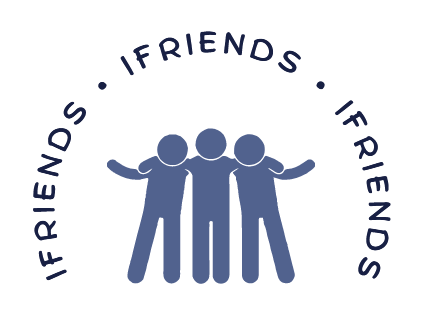
\includegraphics[width=0.5\textwidth]{anexos/logo.png}
\fonte{Os autores.}
\end{figure}
\FloatBarrier

Já a seleção das cores iniciais do sistema traçou um caminho através de um estudo a respeito da psicologia das cores, visto que a equipe se preocupou em passar uma boa experiência até mesmo no quesito visual. Dessa forma, se definiu o azul e suas variações como a cor principal do sistema, já que segundo \citeonline{Tornos2021Sep}, os tons de azul se associam a princípios como: proteção, tranquilidade, fidelidade, compromisso, verdade, estabilidade, criatividade, entre outros. Vale ressaltar que o sistema ainda contará com outras cores, como roxo e algumas de suas variações, cores de sistema: variações de verde e vermelho, e cores neutras: variações de preto, cinza e branco.

Ainda, outro ponto considerado na criação da proposta foi a experiência do usuário final, pois mostrado assim como na \autoref{pesquisa}, a equipe se preocupou em estudar e conhecer melhor as dores deles. Visto que, segundo \citeonline{BibEntry2020Aug}, para tornar essa experiência agradável o sistema deve recorrer aos requisitos do modelo de colmeia desenvolvido por Peter Morville, sendo eles: útil, utilizável, desejável, acessível, confiável, localizável e valioso.

\begin{figure}[htb]
\centering
\caption{Modelo Colmeia}
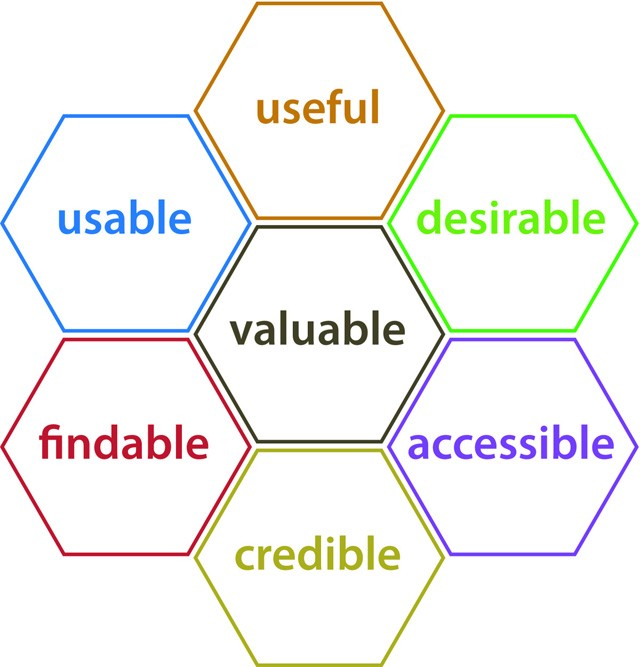
\includegraphics[width=0.4\textwidth]{anexos/modelo_colmeia.jpg}
\fonte{liferay.com}
\end{figure}
\FloatBarrier

%%%%%%%%%%%%%%%%%%%%%%%%%%%%%%%%%%%%%%%%%%%%%%%%%%%%%%%%%%

\section{Pesquisa de viabilidade} \label{pesquisa}
Foi realizada pela equipe uma pesquisa de viabilidade da aplicação, visando verificar se o público-alvo realmente estava sendo atingido, ou seja, se os alunos da instituição possuem interesse na aplicação e pretendem utilizar a mesma como ferramenta cotidiana para auxilia-los durante os estudos.

Para isto, houve a elaboração de um formulário por meio da ferramenta \gls{googleforms}, onde solicitamos que os alunos da instituição respondessem, com sinceridade, dez questões (\autoref{questões}) sobre a proposta. Sua divulgação ocorreu por meio do aplicativo de conversas \gls{WhatsApp}, onde os integrantes da equipe ficaram responsáveis por enviar o endereço de compartilhamento do formulário nos grupos de alunos conhecidos na instituição.

A realização desta pesquisa é de grande importância para a equipe avaliar a proposta que está sendo apresentada e para analisar sua viabilidade por meio dos resultados.
%%%%%%%%%%%%%%%%%%%%%%%%
\subsection{Resultados}

A partir deste formulário, foram recebidas quarenta e cinco respostas acumuladas dentro de um período de cinco dias, e ao final, foi possível constatar as seguintes características na maioria das respostas:

Algumas características do maior grupo que responderam ao questionário são: 

\begin{itemize}
    \item 86,7\% dos estudantes são do ensino médio integrado ao técnico;
    \item 66,7\% dos que sentiram dificuldade ao ingressar no \acs{ifsp}, compartilhou em forma de resposta curta suas experiências (como, adaptação com as atividades, dificuldades em matérias específicas, falta de transparência nas informações institucionais);
    \item 60\% nunca frequentaram ou vão raramente às monitorias;
    \item 85,5\% usariam o sistema e acreditam que o mesmo o ajudaria academicamente;
\end{itemize}

Com base nesses resultados, a equipe entende que a proposta cumpre seu objetivo de atingir os alunos do \acs{ifsp} com o desenvolvimento de uma comunidade de apoio aos assuntos enfrentados durante sua formação. Para pesquisas futuras, foi percebido, com base nas respostas, que uma melhoria na descrição das funcionalidades ajudaria o público-alvo a compreender melhor o objetivo da aplicação. Portanto, é possível validar, futuramente, dores dos usuários com pesquisas de usabilidade após melhores detalhamentos sobre o escopo do sistema.
%%%%%%%%%%%%%%%%%%%%%%%%%%%%%%%%%%%%%%%%%%%%%%%%%%%%%%
\section{Funcionalidades iniciais}

Através da pesquisa de viabilidade e das discussões feitas anteriormente pela equipe, foram elencadas algumas funcionalidades que poderão compor o escopo inicial do projeto, conforme apresentadas nessa sessão. 

\begin{itemize}
\item \textbf{Perguntar e responder questões}: Possibilitar que os usuários respondam e façam perguntas no fórum;

\item \textbf{Gamificação para ganho de reputação a cada reposta dada}: Possibilidade de votar positivamente nas respostas e de ganhar emblemas conforme o aumento da sua reputação;

\item \textbf{Trazer as perguntas mais relevantes na página inicial}: Exibir na página inicial para o usuário, as perguntas mais relevantes sobre temas específicos, tal relevância será considerada por meio da interação recebida. 

\item \textbf{Dividir as perguntas por categorias}: Serão predefinidas de antemão todas as possíveis categorias que podem chegar a ser necessárias na elaboração das perguntas, e caso chegue a faltar alguma, o usuário poderá fazer o uso da categoria ``outros'' que também estará disponível para suprir tal inconveniente. 

\item \textbf{Recorrer a \textit{tags}}: Para auxiliar as categorias, o usuário também poderá recorrer ao uso de \textit{tags}, as \textit{tags} seriam especificações a mais a respeito daquela categoria. Dessa forma, caso o usuário opte pela categoria ``Matemática'', dentro de suas \textit{tags} ele poderá definir, por exemplo, a matéria referente como ``Porcentagem''.

\item \textbf{Divulgação de monitorias no perfil do usuário}: O usuário terá uma seção no seu perfil para mostrar seus eventos de monitorias de determinados assuntos.

\end{itemize}


%%%%%%%%%%%%%%%%%%%%%%%%%%%%%%%%%%%%%%%%%%%%%%%%%%%%%%%%%%%%%%


% ---------------------------------------------------------
% Referências bibliográficas
% ----------------------------------------------------------
\bibliography{referencias,exemplos/abntex2-doc-abnt-6023}

% ----------------------------------------------------------
% Glossário
% ----------------------------------------------------------
%
%
\ifdef{\printnoidxglossary}{
    \addcontentsline{toc}{chapter}{GLOSSÁRIO}
    \printnoidxglossary[style=glossario]
    %\printglossaries
    \cleardoublepage
}{
}
% ----------------------------------------------------------
% Apêndices
% Documentos gerados pelo próprio autor
% ----------------------------------------------------------

% ---
% Inicia os apêndices
% ---
\begin{apendicesenv}

% Imprime uma página indicando o início dos apêndices
\partapendices

% ----------------------------------------------------------
\chapter{Perguntas da pesquisa de viabilidade}
\label{questões}
% ----------------------------------------------------------
\begin{enumerate}
  \item Qual é o seu grau de escolaridade?
  \item Qual é o seu curso?
  \item Você trabalha ou faz estágio?
  \item Você sentiu dificuldade em se adaptar ao entrar no IF?
  \item Descreva como foi a sua experiência (com relação as dificuldades na instituição e no ensino).
  \item Com que frequência você costuma ir às monitorias?
  \item Você usaria um sistema de perguntas e respostas do IF?
  \item Você acredita que uma comunidade de perguntas e respostas te ajudaria na sua vida acadêmica?
  \item De que forma isso faria/não faria diferença para você? (Fique a vontade de responder com toda sinceridade!).
  \item Gostaria de compartilhar mais alguma coisa sobre o tema? Bem, sinta-se a vontade!
\end{enumerate}

\end{apendicesenv}
% ---


\end{document}